\chapter{Algorithmen zur Pfadplanung}
\section{Was sind Algorithmen zur Pfadplanung?}
%Es stellt sich die Frage was ein Pfadplanungsalgorithmus "uberhaupt ist, nach [Lavalle] ist es nicht sinnvoll eine genaue Mathematische Definition abzugeben, sondern das Ziel ist eine generelle Idee zu vermitteln und diese mit Beispielen zu veranschaulichen.
%Als eine Antwort zu der Frage wird eine Turing Maschine beschrieben, da damit die meisten Pfadplanungsalgorithmen modelliert werden k"onnen. Turing Maschinen sind "finite-state-machines" welche informationen als String einlesen, diese verarbeiten und aktzeptieren oder ablehnen k"onnen. 
%Mit einer Erweiterung dieses Konzepts kann am Ende auch ein Pfadplan ausgegeben werden. Das Problem bei der Pfadplanung kommt daher, dass die Maschine auf die Umgebung oft reagieren muss, und informationen die durch Sensoren gegeben werden mit einbeziehen m"ussen. 
%Dadurch gibt es keine klare Trennung von der Umwelt und der Maschine solange nicht alle Daten dem System im Vorhinein bekannt sind.[Lavalle]
%\newline
%Ein Ansatzpunkt w"are ein \"on-line algorithmus" der sich aktiv aktualisiert, aber auch dieser kann nicht die gesamte komplexit"at wiederspiegeln. 

Algorithmen zur Pfadplanung sind schwierig mathematisch pr"azise zu definieren. Ein Ansatz ist eine Definition f"ur einen Algorithmus abzugeben und diese anschlie"send zu erweitern, sodass sie den Anspr"uchen der Pfadplanung entspricht. Nach der Church-Turing These ist ein Algorithmus eine Turing Maschine cite{462,891}. Dieser Definition fehlt aber unter anderem, die Repr"asentation der Interaktion eines Roboters mit der Umgebung, wie es in \ref{lav01} dargestellt wird. Daher wird ein Planer \footnote{Planer (engl. planner)} als ein Algorithmus definiert, welcher einen Plan \footnote{Plan (engl. plan)} konstruiert. Der Planer kann sowohl eine Maschine als auch ein Mensch sein und kann dem Konzept einer Turing Maschine entsprechen. Er ist aber nicht darauf limitiert, sondern kann den Anspr"uchen entsprechend erweitert werden.\cite[~S. 19ff]{Lav06} 

\begin{figure} % Hier lieber eine eigene Kombination an Grafiken
	\centering
	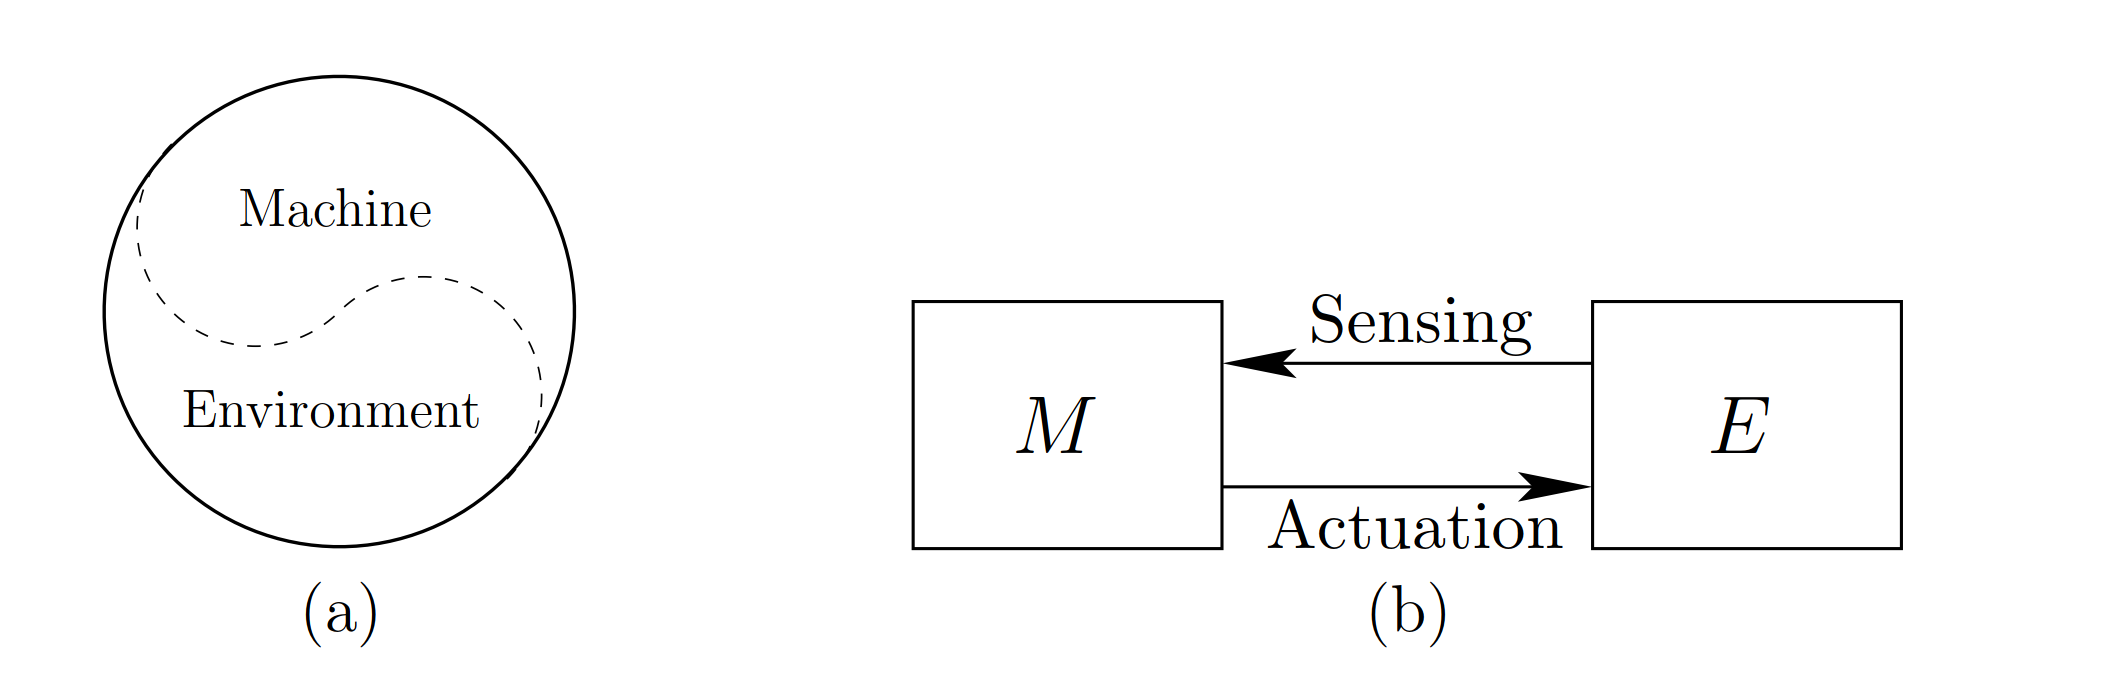
\includegraphics[width=0.6\textwidth]{images/img224.png}
	\caption{Abb. 1.5 von \cite[~S. 20]{Lav06}:  (a) Die Grenze zwischen Maschine und Umgebung ist flie"send, es ist eine Linie die stark in Abh"angigkeit vom Kontext gezogen wird. (b) Ist die Grenze festgelegt, wird angenommen, dass die Maschine M mit der Umgebung U durch Sensorik und den Antrieb interagiert.}
	\label{lav01}
\end{figure}
 



Ein solcher Plan, kann drei unterschiedliche Funktionen erf"ullen. Darunter fallen die Ausf"uhrung \footnote{Ausf"uhrung (engl. Execution)} der Anweisungen in einer Simulation oder durch einen Roboter, die Verbesserung\footnote{Verbesserung (engl. Refinement)} der Eigenschaften in bestimmten Parametern und die hierarchische Einbindung \footnote{Hierarchische Einbindung (engl. Hierarchical Inclusion)} des Plans.
%Ausführung
Pl"ane k"onnen auf zwei weisen ausgef"uhrt werden. Zum einen kann ein Plan als kodierte Eingabe f"ur eine Maschine erstellt werden, welche dadurch programmiert werden kann. Auf diese weise wird die Maschine bei der Ausf"uhrung autonom und kann nicht mehr mit dem Planer interagieren. 
Im zweiten Fall erzeugt der Planer eine Spezialmaschine \footnote{Spezialmaschine (engl. special-purpose machine)}, welche dazu entworfen ist eine Aufgabe zu l"osen.
\newline\\
%Verbesserung
Um einen Plan zu verbessern, wird dieser als Eingabe einem Planer "ubergeben, der daraus einen verbesserten Plan erzeugen soll. 
Anhand von \ref{lav02} wird ersichtlich, wie der gleiche Plan verbessert werden kann, indem verschiedene Aspekte der Problemstellung fokussiert werden.
Die Auswahl der richtigen Kriterien ist schon seit l"angerer Zeit ein Forschungsgebiet in der Robotik, da auch hier Vor- und Nachteile mit verschiedenen Kriterien einhergehen.
\newline\\
%Hierarchische Einbindung
Bei der Hierarchischen Einbindung, wird ein Baum aus Pl"anen erzeugt. Dabei steht an der Wurzel der Hauptplan \footnote{Hauptplan (engl. masterplan)}, welcher andere Pl"ane als Bl"atter in einer Hierarchie einbindet. Ein Plan wird als Aktion betrachtet, die nur als Teil des Gesamtsystem funktioniert. Es wird dadurch erreicht, dass die Abgrenzung zwischen Maschine und Umgebung an verschiedenen stellen gezogen wird.
\newline\cite[~S. 21ff]{Lav06} 

\begin{figure} % Hier lieber eine eigene Kombination an Grafiken
	\centering
	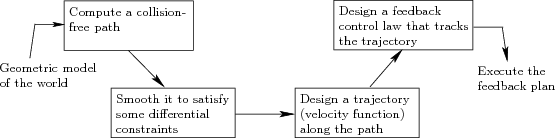
\includegraphics[width=0.6\textwidth]{images/img247.png}
	\caption{Abb. 1.5 von \cite[~S. 20]{Lav06}:  Ein Verbesserungsprozess, der sich in der Robotik bew"ahrt hat.}
	\label{lav02}
\end{figure}

\section{Klassifizierung von Pfadplanungsalgorithmen} % Hier bitte noch ein Bild, das die Unterschiede der einzelnen Klassen sichtbar macht. 
Der Bereich der Pfadplanung ist "au"serst heterogen, da die Umsetzung der Pfadplanung stark von den Vorgaben des Einsatzgebiets abh"angt. 
Es wird Planen in einem diskreten und in einem kontinuierlichen Zustandsraum\footnote{Zustandsraum (engl. state space) Der Zustandsraum beschreibt alle potentiell aufkommenden Zust"ande.} unterschieden. Planen in einem kontinuierlichen Zustandsraum wird Bewegungsplanung genannt, dabei klassifiziert man zwischen Planung mit allen Umgebungsinformationen vorhanden, Planen mit Unsicherheit, sowie Planung mit Bewegungseinschr"ankungen.
Auf die genaue Einteilung der Einsatzgebiete wird in \ref{konti} noch eingegangen, jedoch ist es f"ur das Verst"andnis der Algorithmen wichtig eine Einsch"atzung der verschiedenen Anforderungen zu erhalten. Im folgenden behandeln wir vor allem die diskrete Pfadplanung, da man daran die Grundlagen erkl"aren kann. \cite[~S. 24ff]{Lav06} 

\section{Diskrete Pfadplanung} \label{Kapitel 4.3} % In diesem Kapitel hätte ich gerne noch ein Bild, das das Konzept der diskreten Pfadplanung auf einen Blick veranschaulicht veranschaulicht

Diskrete Pfadplanung dient in der meisten Literatur als Einstiegspunkt. Das kommt davon das der \textit{state space} entweder endlich, oder z"ahlbar unendlich ist.\\
Es m"ussen dadurch keine geometrischen Modelle, oder Bewegungseinschr"ankungen \footnote{Bewegungseinschr"ankungen (engl. differential constraints)} im Entwurf des Algorithmus beachtet werden.
% Der Planer weis "uber alles bescheit, die struktur ist regelmaeßig
Je nach Anforderung werden die drei Teilgebiete \textit{feasible planning} \footnote{feasible planning (Dt. durchf"uhrbares Planen) im folgenden FP}, \textit{optimales Planen} und \textit{Logik basierte Repr"asentation} unterschieden.\cite[~S. 27]{Lav06}\\
% Die vorherrschenden Algorithmen in diesem Bereich, sind der Dijkstra-Algorithmus aus der Graphentheorie und der daraus abgeleitete A*-Algorithmus. Von diesem gibt es noch eine Reihe weiterer Abwandlungen, die alle eine Optimierung auf ein bestimmtes Einsatzgebiet zum Ziel haben. \\
%Wie man diese Optimierung durchf"uhren kann wird im folgenden an verschiedenen Algorithmen erl"autert. 
Optimales Planen unterscheidet sich nur insofern vom feasible planning, als das der gefundene Pfad in verschiedenen Kriterien wie Zeit, Distanz oder auch der Anzahl an Drehungen eines Roboters optimiert werden kann.\cite[~S. 43]{Lav06} \\
Zwischen Zust"anden des \textit{state space} kann durch die Ausf"uhrung von Aktionen gewechselt werden. Die verf"ugbaren Aktionen werden in einem Aktiosraum\footnote{Aktionsraum (engl. action space) } zusammengefasst, au"serdem ist als Teil des Planungsproblem ein Satz von Zielzust"anden\footnote{Zielzust"ande (engl. goal states)} definiert. 
Da ein Zustandsgraph schnell sehr gro"s werden kann, wird dieser meist nicht komplett "ubergeben, sondern diese wird im Laufe des Planungsprozess aufgedeckt.
\cite[~S. 43]{Lav06} \\
Wie man effektiv durch den Zustandsraum navigiert, um einen \textit{goal state} zu erreichen ist das Thema des folgenden Absatz.
\begin{figure}
\centering
\subsection*{Formulierung 4.3 (Discrete Feasible Planning)}
\begin{enumerate}
	\item Ein nichtleerer Zustandsraum $X$, der endlich viele oder z"ahlbar unendlich viele Zust"ande beschreibt.  
	\item F"ur jeden Zustand $x \in X$ , ein endlicher Aktionsraum $U( \, x) \,$.
	\item Eine Zustands"ubergangsfunktion $f$ welche einen Zustand  $f( \, x,u) \, \in X$ f"ur jedes $x \in X$  und $u \in U( \, x) \,$ erzeugt. Die Zustands"ubergangsgleichung ist von $f$ als $x' = f( \, x,u )\, $ abgeleitet.
	\item Ein Anfangszustand $ x_{I} \in X$.
	\item Ein Satz mit Zielzust"anden $X_{G} \subset X$.
\end{enumerate}
\caption{In Anlehnung an Formulation 2.1 von \cite[~S. 29]{Lav06}}
\label{lav03}
\end{figure}
%1. A nonempty state space X, which is a finite or countably infinite set of states.
%2. For each state x ∈ X, a finite action space U(x).
%3. A state transition function f that produces a state f(x, u) ∈ X for every
%x ∈ X and u ∈ U(x). The state transition equation is derived from f as
%x′ = f(x, u).
%4. An initial state xI ∈ X.
%5. A goal set XG ⊂ X.


%
%\begin{algorithm}
%	\caption{Calculate $y = x^n$}
%	\begin{algorithmic}
%		\REQUIRE $n \geq 0 \vee x \neq 0$
%		\ENSURE $y = x^n$
%		\STATE $y \leftarrow 1$
%		\IF{$n < 0$}
%		\STATE $X \leftarrow 1 / x$
%		\STATE $N \leftarrow -n$
%		\ELSE
%		\STATE $X \leftarrow x$
%		\STATE $N \leftarrow n$
%		\ENDIF
%		\WHILE{$N \neq 0$}
%		\IF{$N$ is even}
%		\STATE $X \leftarrow X \times X$
%		\STATE $N \leftarrow N / 2$
%		\ELSE[$N$ is odd]
%		\STATE $y \leftarrow y \times X$
%		\STATE $N \leftarrow N - 1$
%		\ENDIF
%		\ENDWHILE
%	\end{algorithmic}
%\end{algorithm}

\subsection {Feasible Planning} % Hier sollte mit einem Code Beispiel ein allgemeingültiger algorithmus veranschaulicht werden. Darauf kann dann später wieder eingegangen werden und veränderungen im code können mit veränderungen in der Funktionalität in kontakt gesetzt werden.\\
Beim FP werden Algorithmen in Form der in \ref{lav04} gegebenen \textit{Forward Search} verwendet. Diese m"ussen systematisch vorgehen, dass hei"st:
\begin{enumerate}
	\item Bei endlich vielen Zust"anden, m"ussen alle besucht werden. (Zeile 2)
	\item Besuchte Zust"ande m"ussen markiert werden, um wiederholtes absuchen zu verhindern. (Zeile 9)
	\item Bei einem unendlichen Graphen reicht es aus, zu einer L"osung zu kommen, sollte diese vorhanden sein. (Zeile 5)
\end{enumerate} \cite[~S. 32]{Lav06}
\begin{figure}
	\centering
	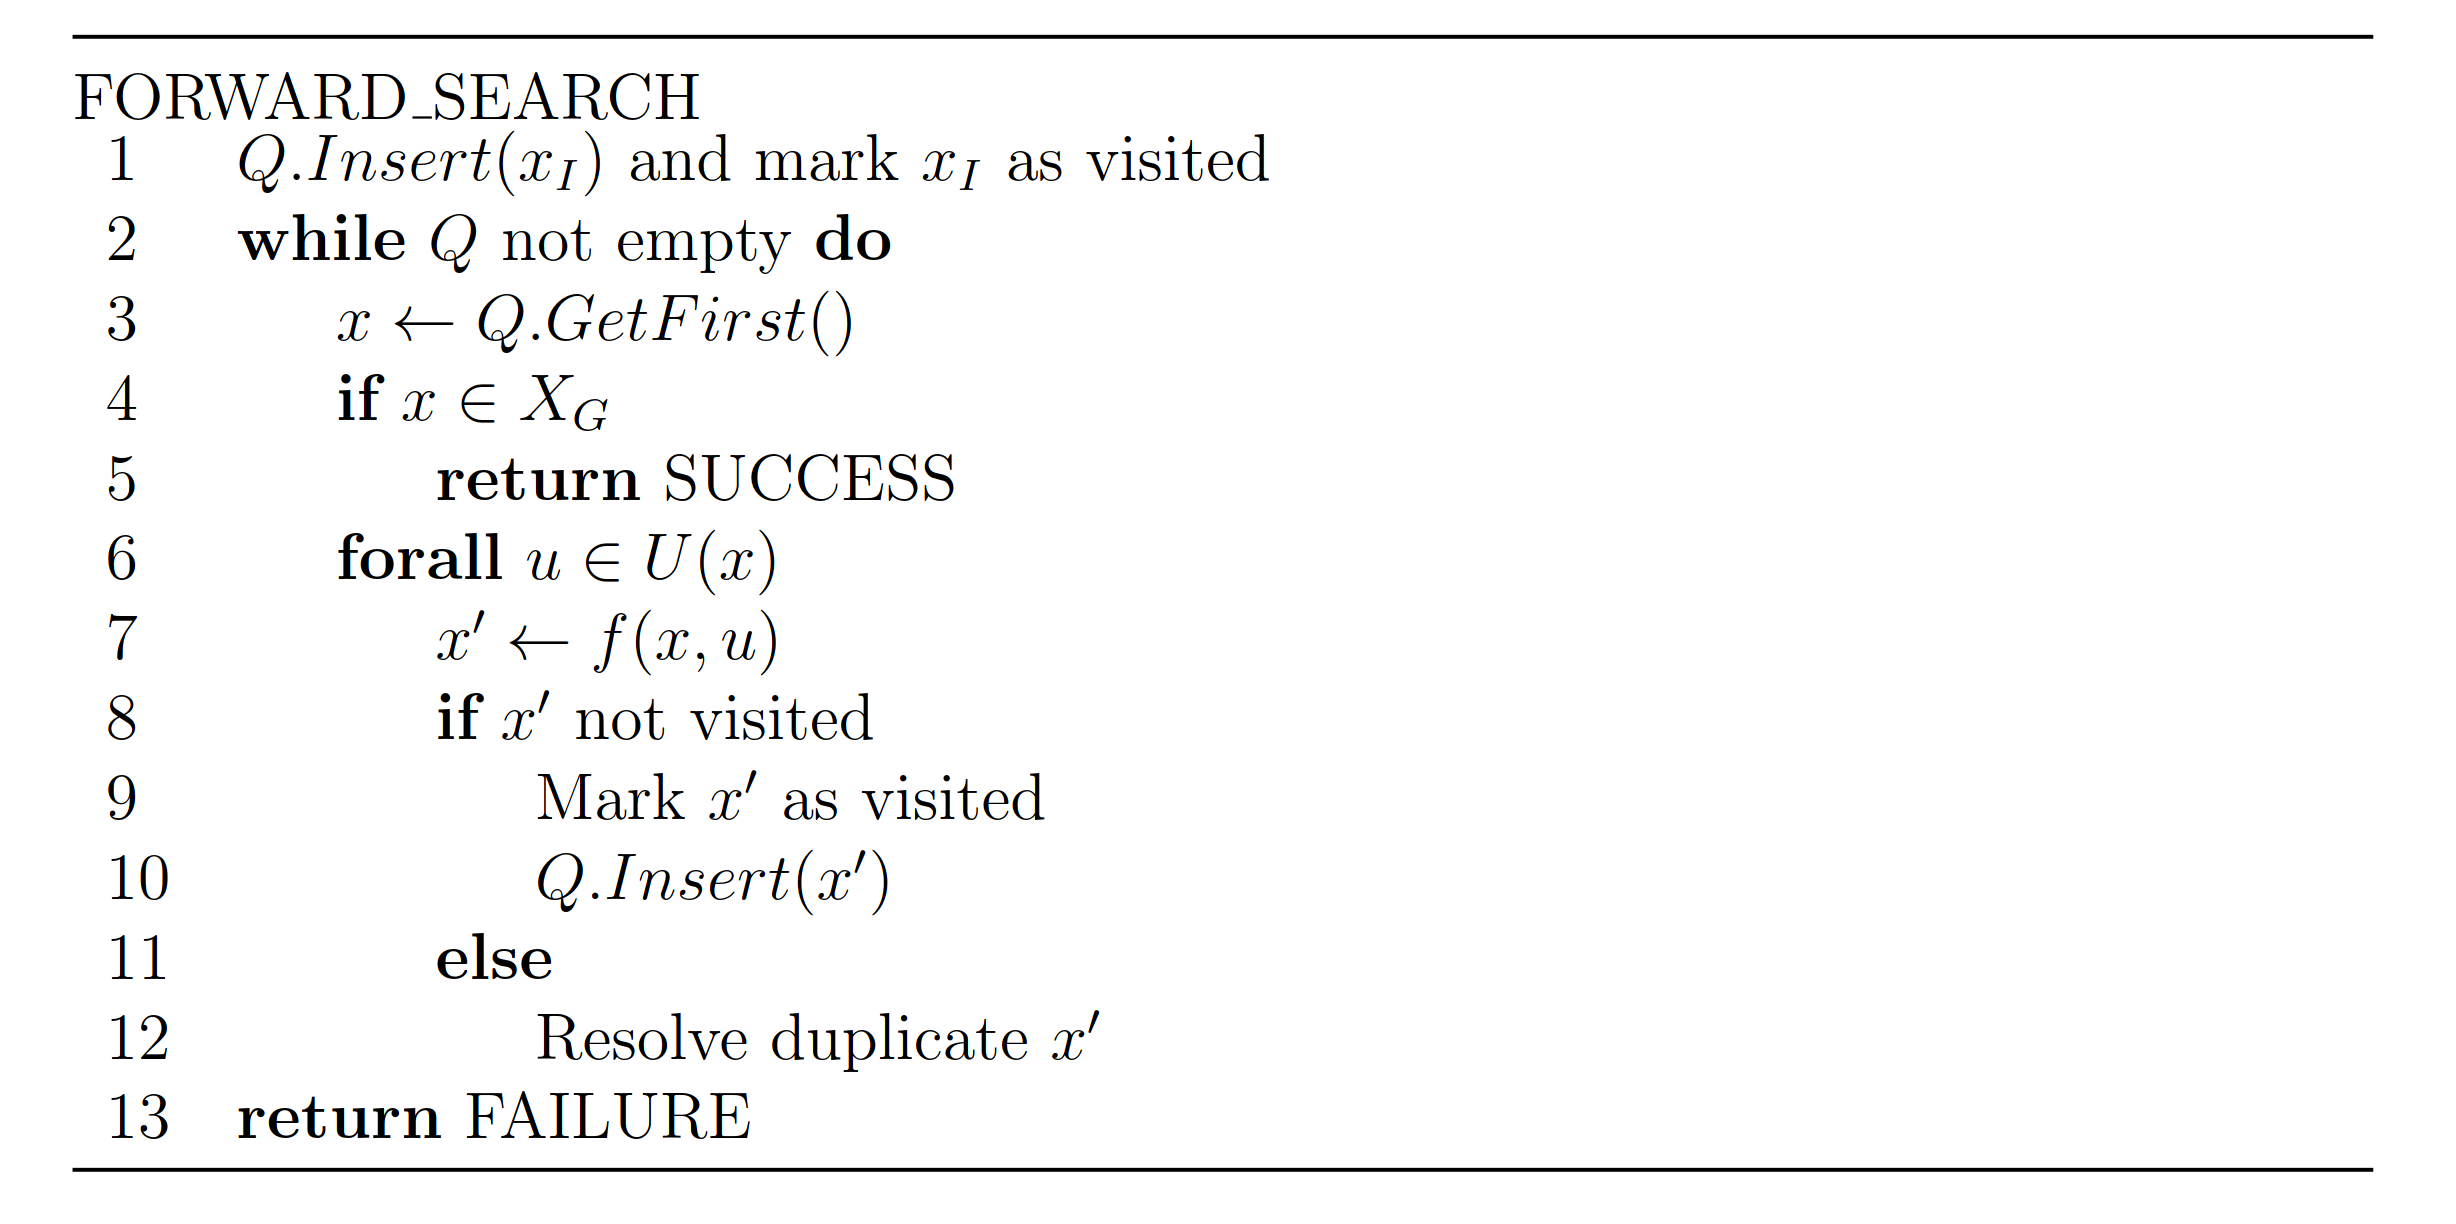
\includegraphics[width=0.9\textwidth]{images/img225.png}
	\caption{Abbildung 2.4 von \cite[~S. 33]{Lav06}:  Eine generelle Schablone f"ur die vorw"arts Suche.}
	\label{lav04}
\end{figure} 

Felder k"onnen drei Zust"ande einnehmen:
\begin{enumerate}

\item \textit{unentdeckt}: wurde noch nicht besucht und ist daher auch noch nicht bekannt.
\item \textit{tot}: kann nichts mehr zur Suche beitragen, da alle angrenzenden Felder entdeckt wurden.
\item \textit{lebend}: hat noch mindestens ein Nachbarfeld das unentdeckt ist.  
\end{enumerate} \cite[~S. 33]{Lav06}


In der Warteschlange \footnote{Warteschlange (engl. priority queue)}, Abbildung \ref{lav04} Zeile 1, werden die n"achsten Felder gespeichert. Dessen Sortierung hat einen gro"sen Einfluss auf das Verhalten des Algorithmus. 
	\begin{itemize}
		\item Die einfachste Variante ist \textit{First-In First-Out} \footnote{FI-FO - Das am l"angsten wartende Element zuerst}, hier entsteht eine kreisf"ormig expandierende Suche. Dies wird im \textbf{Breath-first} Suchalgorithmus verwendet. Er ist systematisch und leicht zu kontrollieren, jedoch verschwendet er relativ viele Suchzyklen.\cite[~S. 35]{Lav06}
		\item Mit \textit{Last-In First-Out}\footnote{LI-FO - Das neuste Element zuerst}, entsteht eine aggressive Expansion in eine bestimmte Richtung. 
		Dies w"are ein erstrebenswertes Verhalten, die Richtung kann aber mit LI-FO nicht kontrolliert werden. Der \textbf{Depth-first} Algorithmus setzt das ein, er ist aber aber nur bei endlich vielen Knoten systematisch. \cite[~S. 36]{Lav06}
		\item Der \textbf{Dijkstra} Algorithmus vergleicht im Laufe der Suche Aktionen mit einander, und erstellt so eine Warteschlange die Knoten mit besseren Chancen bevorzugt. Im normalfall sucht er solange bis der optimale Pfad gefunden wurde. Das Vorgehen ist weitgehend bekannt und kann bei \cite[~S. 36]{Lav06} nachgelesen werden.
		\item Der \textbf{A*-Suchalgorithmus}\footnote{A-Stern gesprochen} erweitert das Konzept um eine Sch"atzfunktion, welche die gesch"atzten Kosten bis zum Ziel beschreibt.
		$$f( \, n ) \, = g ( \, n ) \, + h ( \, n ) \,$$
		So werden Knoten bevorzugt, welche die Suche m"oglichst schnell, n"aher zum Ziel bringen. Das daraus entstehende Verhalten zeichnet sich dadurch aus, dass der Algorithmus solange in Richtung des Ziels sucht, bis er auf ein Hindernis st"o"st. Erst dann versucht dieses zu umgehen. Es wird garantiert, dass immer der optimale Pfad gefunden wird.\cite[~S. 37]{Lav06}
	\end{itemize}
Um den gefundenen Weg zu rekonstruieren m"ussen die Vorg"angerknoten jedes Knoten gespeichert werden. Dies w"urde man in \ref{lav04} Zeile 7 vornehmen. 


%Simon fährt fort
\section{Planung mit kontinuierlichem Zustandsraum} \label{konti}
Lorem ipsum dolor sit amet, consetetur sadipscing elitr, sed diam nonumy eirmod tempor invidunt ut labore et dolore magna aliquyam erat, sed diam voluptua. At vero eos et accusam et justo duo dolores et ea rebum. Stet clita kasd gubergren, no sea takimata sanctus est Lorem ipsum dolor sit amet. Lorem ipsum dolor sit amet, consetetur sadipscing elitr, sed diam nonumy eirmod tempor invidunt ut labore et dolore magna aliquyam erat, sed diam voluptua. At vero eos et accusam et justo duo dolores et ea rebum. Stet clita kasd gubergren, no sea takimata sanctus est Lorem ipsum dolor sit amet.

 
%%oder einer Grafik die ich noch schreiben muss. 
%\section{Bewegungsplanung}
%% Die Planung muss zus"atzlich noch die Bewegung in der Umgebung in betracht ziehen. 
%\subsection{Sampling-Based Motion Planning}
%\subsection{Combinatorial Motion Planning}
%\section{Planen mit Unsicherheit}
%% Hier kommt noch unsicherheit in der Umgebung hinzu, also auch dynamische Systeme
%\subsection{Entscheidungstheorie}
%\subsection{Planen mit Unsicherheiten in der Sensorik}
%\section{Planen mit Differentialen Einschr"ankungen}
%% Hier müssen bewegungseinschr"ankungen die durch den Verwendeten Roboter einhergehen beachtet werden. 
%\subsection{Sampling-Based Planning under Differential Constraints}
